\documentclass[convert]{standalone}
\usepackage[utf8]{inputenc}
\usepackage{amsmath}
\usepackage{amsfonts}
\usepackage{amssymb}
\usepackage{tikz}
\usetikzlibrary{calc}

%\usepackage[left=2.00cm, right=1.50cm]{geometry}

\begin{document}

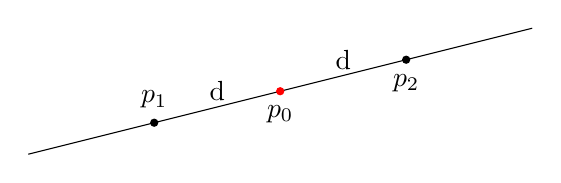
\begin{tikzpicture}[scale=0.8]
\tikzset{mark coordinate/.style={ %
		inner sep=0pt,
		outer sep=0pt,
		minimum size=3pt,
		fill=#1,
		circle %
	}
}
\draw (-4,-1) -- (4,1);
\draw[thick] (0,0)  coordinate [mark coordinate=red,label={270:$p_0$}]   (orig);
\draw[thick] (-2,-.5)  coordinate [mark coordinate=black,label={:$p_1$}]   (c);
\draw[thick] (2,.5)  coordinate [mark coordinate=black,label={-90:$p_2$}]   (c);
\node at (1,.5) {d};
\node at (-1,0) {d};
\end{tikzpicture}
%\end{center}


\end{document}
